Tudo começou quando uma renomada coruja usando chapéu e monóculo chegou.

``É um prazer recebê-lo no Grande Hotel Infinita'', disse Henrietta. ``Um lugar onde a busca incessante se desfaz, para que você descanse e encontre paz.''
%``Um lugar onde a busca incessante fica para trás, onde você pode descansar e deixar o redemoinho dos turbulentos sonhos para trás.''

A coruja respondeu com um pedido peculiar: ``Obrigado, minha cara. Eu gostaria de um quarto no primeiro andar, pois tenho um medo terrível de altura.''

``Os quartos do primeiro andar estão completamente cheios'', suspirou Henrietta. Era um problema comum, já que os hóspedes geralmente não gostavam de ter que usar as escadas. Mas, tentando ser o mais amigável e cuidadosa possível, ela acrescentou, ``Mas não se preocupe!''

Para acomodar este hóspede eminente, ela ligou para o distinto leão-marinho e, da maneira mais delicada, pediu-lhe que se mudasse do Quarto 1 no primeiro andar para o Quarto 1 no segundo andar. O leão-marinho prontamente concordou.

\vfill
\begin{center}
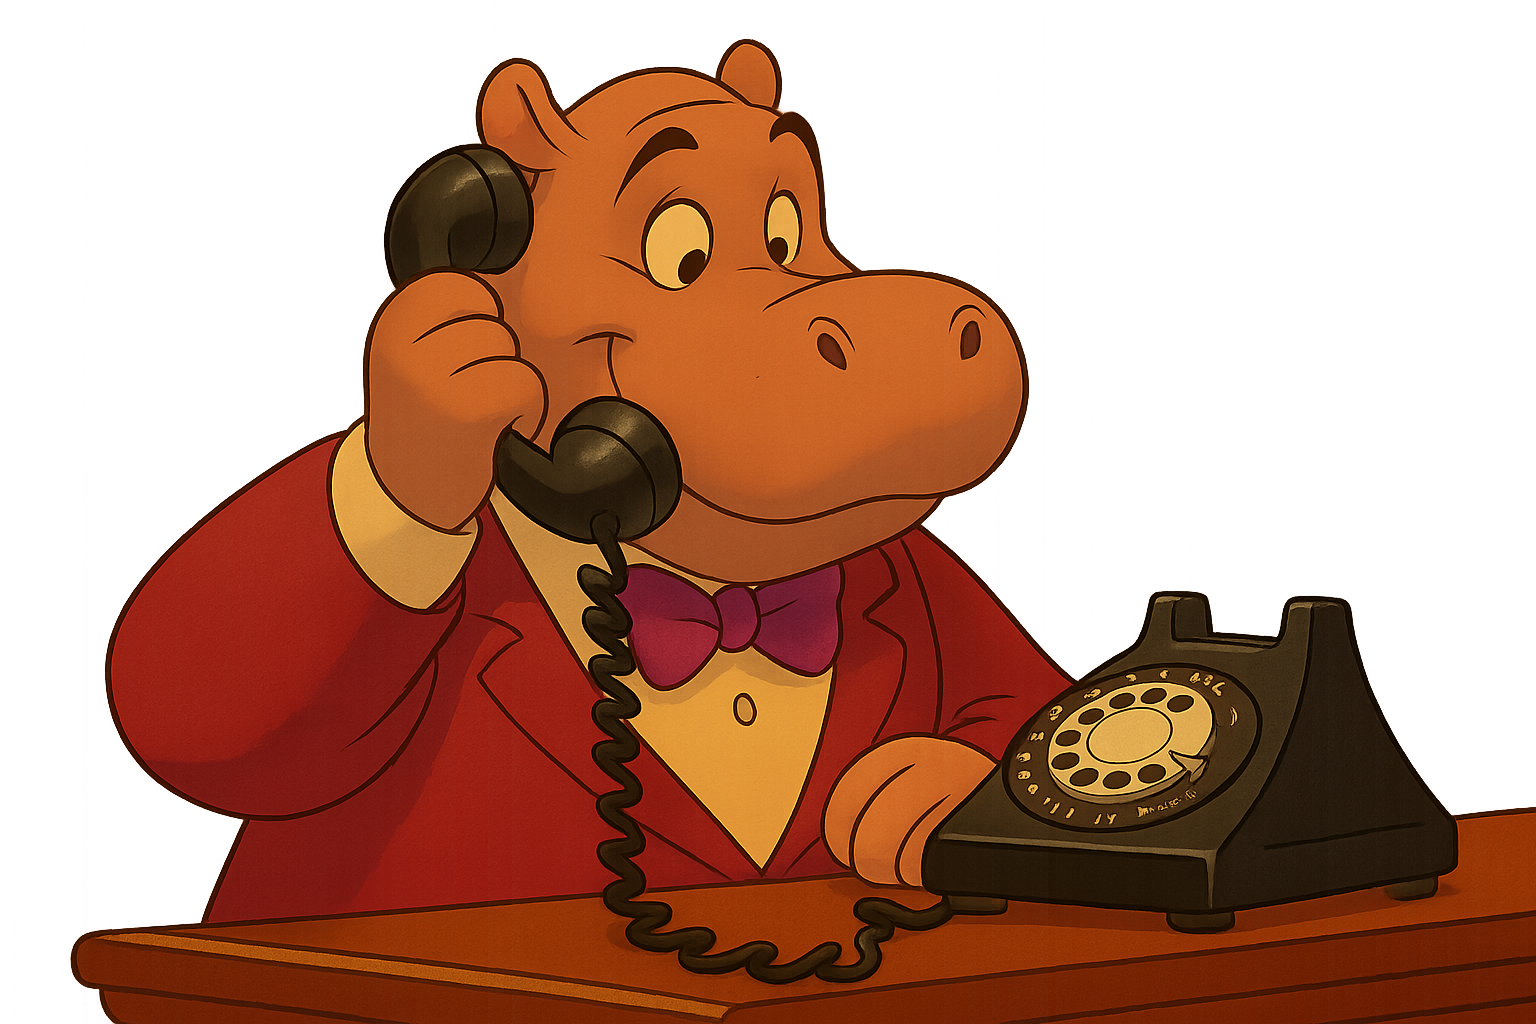
\includegraphics[width=0.5\textwidth]{images/telephone.png}
\end{center}

\clearpage
\includepdf[pages={1},
            pagecommand={\thispagestyle{fancy}}, % Apply your custom 'fancy' style
            fitpaper=true,
            noautoscale
           ]{elevator.pdf}

%Para acomodar este hóspede eminente, ela chamou o distinto leão-marinho e, da maneira mais delicada, pediu-lhe que se mudasse do Quarto 1 no primeiro andar para o Quarto 1 no segundo andar. O leão-marinho prontamente concordou. 
Bernard rapidamente pegou os pertences do leão-marinho e os moveu para o andar de cima usando o pequeno elevador de carga.

``Bernard irá ajudá-lo a chegar ao seu novo quarto imediatamente!'' acrescentou Henrietta.

A coruja ficou encantada em pegar o quarto recém-vago no primeiro andar, e Bernard rapidamente trouxe sua bagagem.

Poucos minutos depois, uma graciosa girafa de cachecol e meias compridas apareceu. Com um olhar deslumbrante, ela entrou, observando cada detalhe do grande hotel, e com a cabeça erguida, quase a bateu no lustre central. Bernard, vendo Henrietta se preparando para mover a coruja, sugeriu: ``Vamos mover o hóspede do Quarto 2! A coruja acabou de se acomodar e tem medo de altura.'' Henrietta concordou. A girafa, mostrando-se agradecida, disse: ``Que gentileza a sua! Assim não precisarei me esforçar subindo e descendo as escadas infinitas!'' Bernard rapidamente pegou os pertences dela, e ela se acomodou feliz em seu novo quarto.

\vfill
\begin{center}
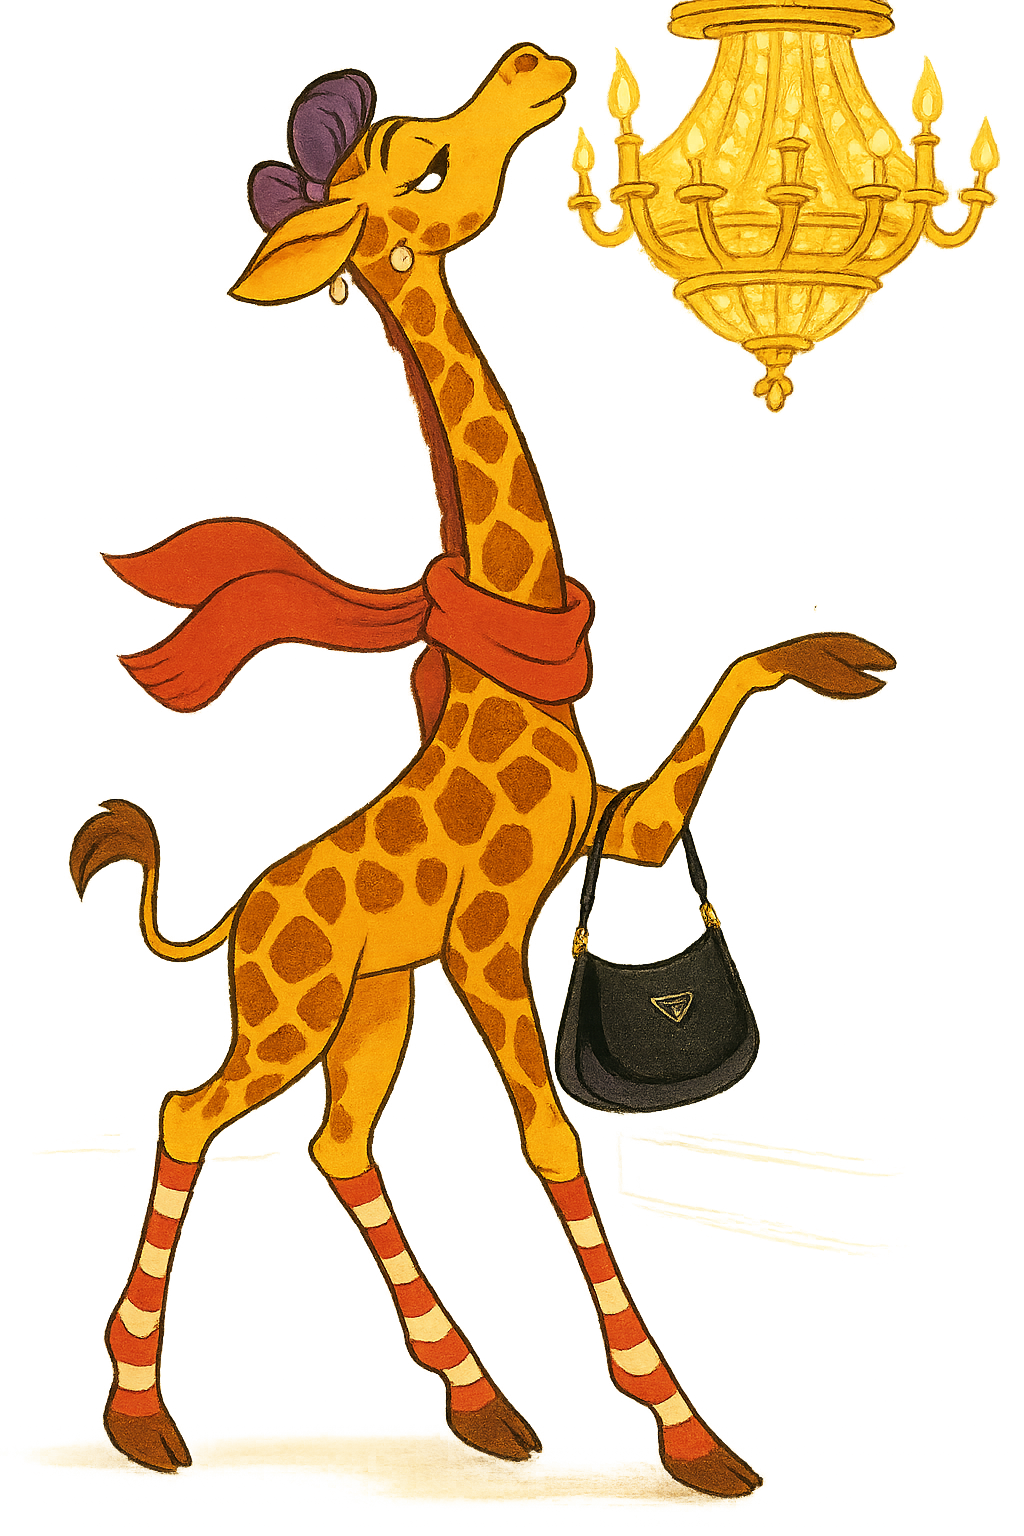
\includegraphics[width=0.45\textwidth]{images/giraffe.png}
\end{center}

\clearpage
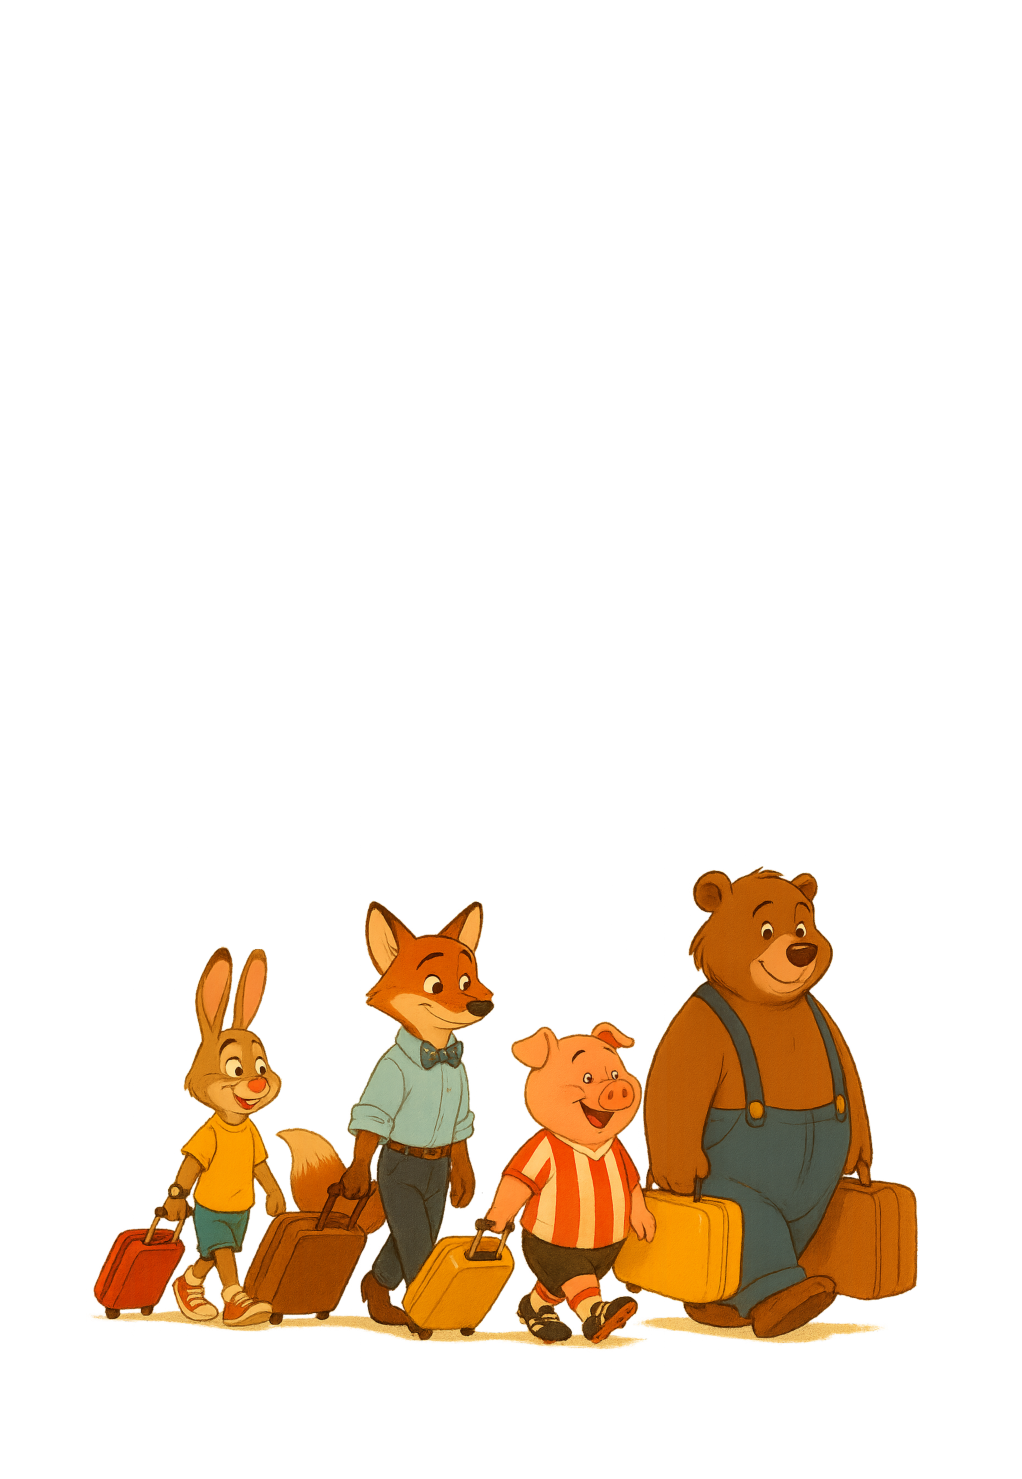
\includepdf[pages={1},
            pagecommand={\thispagestyle{fancy}}, % Apply your custom 'fancy' style
            fitpaper=true,
            noautoscale
           ]{checkinanimals.pdf}

Ao longo do dia, mais e mais hóspedes animais chegaram: um coelho com um relógio de pulso, uma raposa com uma gravata-borboleta, um porco com chuteiras de futebol e um urso com suspensórios. Cada vez, Bernard e Henrietta repetiam seu sistema inteligente, movendo o próximo hóspede do primeiro andar para o segundo, sempre para o mesmo número de quarto. Era uma solução engenhosa para um problema peculiar. No final do dia, eles haviam recebido um total de 54.907 novos hóspedes, e parecia que todos estavam bem acomodados... mas era apenas o início de uma noite caótica.

